\graphicspath{ {./figures/cGAN_figures/} }

\zzcommand{\distRegions}{\Tilde{x}}

\chapter{Automatic generation of coral reef islands}
\label{chap:coral-island}
\teaser{
	\centering
	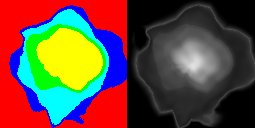
\includegraphics[width=0.6\linewidth]{terrainGAN.png}
	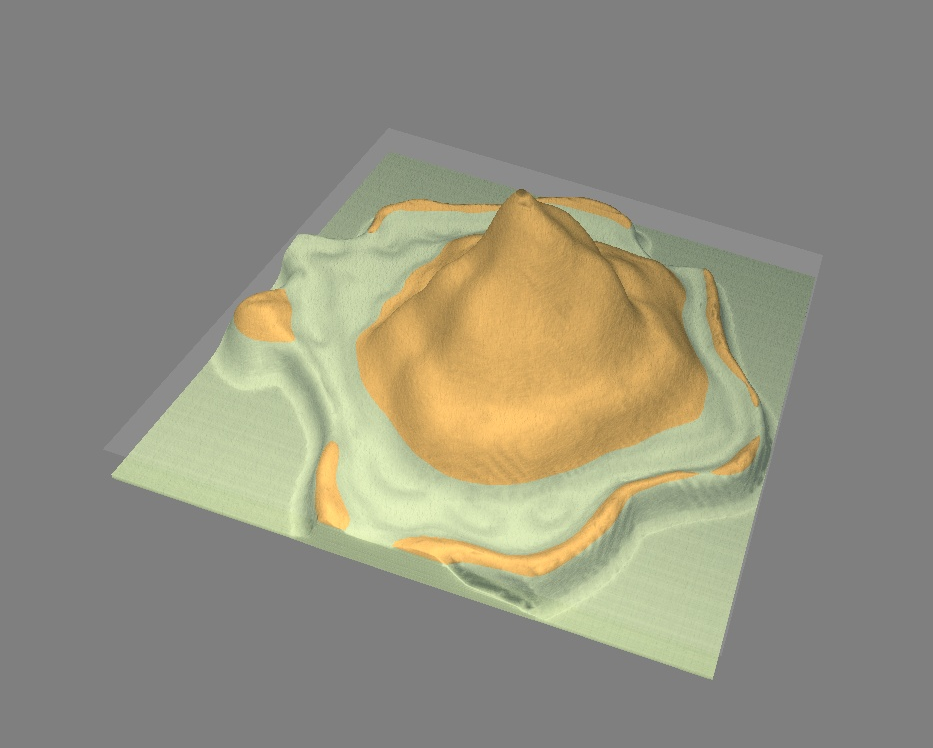
\includegraphics[width=0.3\linewidth]{terrainGAN_result.png}
	\caption{Caption.}
	\label{fig:teaser_cGAN}
}

\abstract 
In this chapter, we propose a procedural method for generating single circular volcanic islands using user sketching from two perspectives: a top view, which defines the island's shape (horizontal dimensions), and a profile view, which outlines its elevation and terrain (vertical dimensions). These perspectives, commonly used in geological and remote sensing domains, are complemented by a user-defined wind field, applied as a distortion field to deform the island's shape, mimicking the effects of wind and waves on the long term. We then model the growth of coral on the island and its surronding in a second time [???] to construct the reef following biological observations. Based on these inputs, our method generates a height field of the island. This algorithm is capable of creating many different island models, and we have generated thousands of exemplars to compose the dataset used for training a conditional Generative Adversarial Network (cGAN). By applying data augmentation, the cGAN allows for even greater variety in the generated islands, providing users with more control over the shape and structure of the final output.
\pagebreak 

\minitoc

\section{Introduction}
\label{sec:coral-island_introduction}

Coral reef islands are formed through a dynamic interplay of volcanic activity, coral growth, and long-term geological processes. These islands begin as volcanic landmasses, created when magma from the Earth's mantle erupts through the ocean floor and builds up layers of volcanic rock, eventually rising above sea level. In tropical waters, these volcanic islands create ideal conditions for coral reefs to develop. Corals, thriving in the shallow, sunlit waters around the island, initially form fringing reefs attached to the island's coastline.

As time passes, the volcanic island undergoes subsidence, a slow sinking process caused by the cooling and contraction of the Earth's crust beneath the island. In response to this subsidence, corals continue to grow upward, maintaining their position within the photic zone, where sunlight supports their survival. This upward growth leads to the formation of barrier reefs, which become separated from the island by a lagoon as the island sinks further.

Eventually, the volcanic island may submerge completely beneath the ocean's surface, leaving only the coral structure visible above water. This process results in the formation of atolls, which are ring-shaped reefs encircling a central lagoon. Over geological time, the physical structure of the island evolves from a prominent volcanic peak to a coral-dominated reef system, shaped by the combined forces of subsidence, coral growth, and erosion.

% 
Charles Darwin's subsidence theory, developed from his observations in \citep{Darwin1842}, remains one of the most widely accepted explanations for the formation of coral reef islands. Darwin proposed that coral reefs form around volcanic islands that slowly subside over time due to geological processes. As the volcanic island sinks, coral reefs grow upward, maintaining their position near the surface of the ocean. This theory explains the transition from fringing reefs attached to the island's coast, to barrier reefs separated by a lagoon, and finally to atolls, where the volcanic island has completely submerged, leaving only the coral structure visible above water.

While other theories, such as John Murray's growth on submerged mountains \cite{MurrayCoralTheory} [CITATION] and Reginald Daly's sea level change theory \cite{Daly1915}, have also been proposed to explain coral reef formation, Darwin's subsidence theory remains the most widely supported due to its ability to account for the full evolution of coral islands, from volcanic landmasses to atolls, iven if it has been recently partially disproved by \citep{Droxler2021} [ADD DETAILS]. Its simplicity and focus on the relationship between subsidence and coral growth make it especially well-suited for computational modeling.

In our approach, we translate the core principles of Darwin's theory into a procedural generation model, simulating the gradual sinking of volcanic islands while coral reefs grow to keep pace with changing sea levels. This allows us to realistically model the transformation of islands from volcanic landmasses to coral-dominated atolls. By capturing this interplay, we can procedurally generate a wide variety of island structures that reflect real-world geological processes.

%

Simulating the formation of coral reef islands presents significant challenges due to the complex interplay of geological, environmental, and biological factors. One major difficulty lies in capturing the long-term subsidence of volcanic islands, which occurs over millions of years, while simultaneously modeling the upward growth of coral reefs that rely on environmental conditions such as water depth, temperature, and sunlight. This combination of slow geological processes and dynamic biological growth is difficult to replicate in a computational model.

Additionally, the biological aspects of coral growth are inherently tied to environmental factors. Coral reefs grow only within a specific range of water depth and sunlight, and their growth patterns are affected by the health of the reef ecosystem and the availability of resources. Accurately modeling these biological dependencies in a procedural system is challenging, as the factors governing coral reef development are difficult to generalize.

Existing terrain generation methods, such as Perlin noise-based algorithms or uplift-erosion models, are often ill-suited for these processes. While they can generate natural-looking landscapes, they do not account for the unique geological and biological interactions that govern coral island formation. Capturing these dynamics requires a balance between realism and procedural flexibility, allowing for both accurate simulation of natural processes and intuitive user control.

%

To address these challenges, we present a procedural generation tool that simulates the formation and evolution of coral reef islands by integrating both geological and biological processes. Our approach allows users to control the island's shape and structure through intuitive sketching interfaces, while the tool models subsidence, coral growth, and environmental deformation.

The generation process begins with two user-defined inputs: a top view to outline the island's overall shape and a profile view to define its elevation and terrain contours. These inputs serve as the foundation for creating a height field of the island. Additionally, a wind deformation field allows the user to simulate the effects of wind and waves, reshaping the island's structure in a way that mimics natural erosion processes.

To enhance flexibility and allow for more complex, non-circular island structures, we incorporate a conditional Generative Adversarial Network (cGAN) into the generation process. The cGAN is trained on a dataset of islands generated by the initial algorithm, augmented to introduce a wider variety of shapes and features. This machine learning component allows for the automatic generation of diverse island models, removing some of the constraints of the initial procedural algorithm such as strictly radial symmetry while maintaining user control over key aspects of the design.

By combining user input with the adaptive power of the cGAN, our tool generates plausible coral reef islands that evolve from volcanic landmasses to coral-dominated atolls, capturing both geological and environmental processes.



\section{Overview}
Our system for generating coral reef islands combines user-driven sketching, procedural techniques, and deep learning to create realistic and varied island terrains. The process begins with the user sketching key features of the island, such as its overall shape and profile. This sketching process allows the user to define the layout of the island in an intuitive way, providing control over the placement of important elements like the island borders, beaches, lagoons, and coral reefs.

[ADD DETAILS ON THE SIMULATION PART]

Once the user's sketch is complete, the system converts these high-level features into a labeled map, where each pixel is assigned to a specific region of the island. This map serves as the input to a conditional Generative Adversarial Network (cGAN), which is responsible for generating the fine details of the terrain. The cGAN has been trained on a dataset of island examples generated by the initial procedural algorithm, allowing it to produce realistic terrains that reflect the user's design while introducing natural variation and complexity.

By conditioning the cGAN on the user-defined map, the system maintains the overall structure and regions specified in the sketch, while generating realistic transitions between different areas (such as beaches, lagoons, and the island's interior). The use of deep learning, in combination with procedural techniques, allows the system to create coral islands that are both geologically plausible and tailored to the user's input.

This method provides a simple and flexible approach to island generation, enabling the creation of diverse island structures that reflect real-world geological processes, such as volcanic subsidence and coral reef growth.



\section{Related works}
Procedural generation of terrain has been a well-researched area in computer graphics and simulations, where the goal is to create large, realistic landscapes with minimal manual input. Various methods have been developed over the years to generate terrains automatically, from noise-based approaches to physically-based erosion simulations, sketch-driven methods, and more recently, deep learning techniques.

However, each of these techniques has its strengths and limitations, particularly when it comes to modeling coral reef islands. Coral islands present unique challenges due to the combination of long-term geological processes (such as subsidence and coral reef growth) and environmental interactions (like erosion caused by wind and waves). In this section, we review the key techniques that have been applied to terrain generation, highlight their limitations for coral island formation, and position our work as an approach that addresses these challenges.

\subsection{Noise functions}
% Noise functions
Noise-based procedural generation remains one of the most widely used techniques for creating natural-looking terrains. Introduced by Ken Perlin, the Perlin noise and Simplex noise are foundational algorithms that generates pseudo-random yet continuous variations across a grid, producing terrain features that resemble organic landscapes \cite{Perlin1985,Perlin2001}.

Beyond basic noise functions, more advanced techniques, such as Fractal Brownian Motion (FBM), are commonly used to add additional detail to terrains. FBM combines multiple layers, or "octaves," of noise at different frequencies, creating terrains with finer details and more realistic features. Noise functions are often paired with falloff maps to generate island-like terrains, where the height of the terrain gradually decreases toward the edges, mimicking the appearance of coastlines and providing a simple way to create basic island shapes.

Despite their widespread use, noise-based methods have significant limitations when applied to the simulation of coral reef islands. While these techniques excel at producing large, varied landscapes quickly, they lack the geological accuracy needed to model real-world processes like volcanic subsidence and coral growth. These approaches generate random patterns, but are disconnected from the actual physical processes that govern coral island formation.

Our approach goes beyond the randomness of noise-based generation by incorporating real-world geological and biological processes into terrain formation. Specifically, we model the gradual subsidence of volcanic islands and the upward growth of coral reefs, which are essential for representing the long-term evolution of coral reef islands. By integrating these processes into the generation algorithm, we create terrains that are not only more realistic but also allow for user control. This blend of user input and geological grounding provides a more accurate and flexible approach to modeling coral reef islands, addressing the limitations inherent in traditional noise-based techniques.

\subsection{Erosion simulation}
% Erosion simulation
While noise functions generate random, natural-looking terrain, they often fail to capture the physical processes that shape real landscapes over time. To address this limitation, erosion simulations model how natural forces such as water flow and gravity wear down terrain features, creating valleys, river networks, and other detailed landforms. These simulations are particularly effective at representing mountainous landscapes, where erosion gradually sculpts the terrain over long periods of time, typically on the scale of hundreds to millions of years.

Erosion simulations often use models like the Stream Power Law to describe how water erodes higher elevations and deposits sediment in lower areas. The rate of erosion depends on factors such as slope steepness and water flow, with steeper slopes and greater water volumes leading to faster erosion. Over time, these processes create detailed and realistic terrain features like river valleys and erosion channels. Erosion models are iterative, simulating the gradual shaping of landscapes by continuously balancing forces like erosion and uplift, as seen in the work of \cite{Cordonnier2016,Cordonnier2017a}. Their model simulates how tectonic forces uplift terrain, which is then eroded away over thousands of years. Similarly, \cite{Schott2023} and \cite{Tzathas2024} refined the Stream Power Law to generate realistic slopes and ridges through these long-term geological processes.

Despite their effectiveness in modeling large-scale terrain evolution, erosion simulations are limited when it comes to representing environments that are shaped by dynamic biological processes. Coral reefs, for instance, grow and adapt to changing environmental conditions on a much shorter timescale than geological erosion. While erosion models simulate terrain changes over millennia, coral growth responds more dynamically to factors like water depth, light availability, and temperature on scales ranging from years to decades. These biological factors are difficult to incorporate into traditional erosion models, which are designed to simulate the slow, steady forces of water and gravity. Recent works however take into account biologic factors in the erosion simulation \cite{Cordonnier2017b} [CITATION DEADWOOD DE GUERIN 2024] [ADD DETAILS, WHAT IT CAN OR CAN'T DO, PROBLEM OF TIME].

Our approach builds on the concept of terrain evolution by integrating the geological and biological dynamics that shape coral reef islands. Instead of focusing solely on erosion, which is primarily a surface-level process, we model the subsidence of volcanic islands over geological time and the simultaneous growth of coral reefs that adapt to the changing sea levels. Coral reefs must grow upward to remain within the photic zone, a process that unfolds on shorter timescales than those captured by standard erosion simulations. Furthermore, we introduce wind deformation to simulate the effects of environmental forces like wind and waves, which reshape the island's structure. This combination of long-term geological processes and short-term biological responses provides a more comprehensive simulation of coral reef island formation, capturing both the slow subsidence of volcanic landmasses and the rapid adaptability of coral ecosystems.

\subsection{Sketching}
% Sketching

In procedural terrain generation, sketch-based approaches allow users to directly interact with and shape landscapes through intuitive sketching interfaces. These methods enable users to define key terrain features such as mountains, valleys, and coastlines by drawing them in a two-dimensional canvas, which are then translated into 2.5D terrains. Sketching provides a high level of artistic control, making it especially useful in creative applications such as video games and simulations, where user-defined terrain features are prioritized.

Sketch-based systems offer great flexibility, allowing users to directly define specific elements of the landscape according to their needs or preferences. For instance, \citep{Gain2009} introduced a multi-perspective sketching system that allows users to generate detailed landscapes by sketching from different angles. This method provides more control over the terrain's shape than traditional noise-based generation methods. Similarly, \citep{Tasse2014} explored sketching from the player's viewpoint, allowing users to dynamically define height information from within the virtual environment, creating an interactive terrain design experience.

Sketching has also been extended to geological modeling. \citep{Patel2021} proposed a system where users can interactively model underground layers by sketching subsurface structures. This provides a powerful tool for geologists and designers who need to model complex, multi-layered terrains, offering more control over both the surface and the subsurface.

In our work, we leverage the flexibility of sketching to define the key features of coral reef islands, such as the island shape, lagoons, and coral reefs, in a vectorized format. This is particularly important for modeling underwater and island landscapes, where these features are not simply surface elements but part of an evolving geological structure. By using sketches, we retain the semantic information of where the island and coral regions are located, which allows us to later apply our simplified model of Darwin's subsidence theory.

Rather than focusing on detailed long-term or short-term evolution, our method adapts sketching to the unique requirements of island and underwater landscapes. Once the user defines the terrain layout through sketching, we apply a simplified subsidence model, where the volcanic island gradually sinks and coral reefs grow in response, remaining close to the water surface. This process provides a framework for simulating the evolution of the landscape in a geologically plausible manner.

The key advantage of sketching in our system is that it combines the artistic control provided by traditional sketching methods with the ability to handle the geological processes specific to coral reef islands. By preserving the vectorized information from the sketch, we can accurately place and evolve features like lagoons and coral reefs, ensuring that the resulting terrain reflects both the user's design intent and the geological dynamics at play.

\subsection{Deep learning}
% cGAN

In recent years, deep learning has become a innovative [MEH... "GAME CHANGER" OR SOMETHING LIKE THIS] tool in computer graphics, image processing, and procedural content generation. Deep learning refers to a class of machine learning techniques that use artificial neural networks with multiple layers to model complex patterns in data. By training these networks on large datasets, deep learning models can learn to generate new, realistic data by identifying the underlying relationships between inputs and outputs.

In terrain generation, deep learning is particularly well-suited for tasks that require the creation of complex, natural-looking landscapes. Traditional procedural generation techniques like noise functions and erosion simulations can be powerful, but they often struggle to produce the complexity and realism of natural terrains due to their reliance on predefined rules and algorithms. In contrast, deep learning models, especially Generative Adversarial Networks (GANs), can learn from real-world data, enabling them to generate realistic terrains that mimic the diversity and complexity found in nature.

GANs are a particularly effective deep learning architecture for terrain generation. A GAN consists of two neural networks: a generator, which creates new data samples, and a discriminator, which evaluates whether the generated samples are real or fake compared to a set of training data. Through this adversarial process, the generator gradually improves its ability to produce realistic examples, while the discriminator becomes better at distinguishing real from fake data. This feedback loop allows GANs to generate highly realistic and detailed terrain features by learning from large datasets of existing terrains.

In terrain generation, GANs have been applied to generate diverse landscapes by learning the patterns and features found in real-world terrains. For example, \citep{Guerin2017} demonstrated how GANs can be used to transform 2D sketches into 3D terrains by training the network on a dataset of terrain features, allowing the system to generate new landscapes based on simple user input. GANs are particularly well-suited for this task because they can capture the subtle details of terrain that would be difficult to model explicitly, such as the natural flow of elevation or the transitions between different terrain types.

A variant of GANs, known as Conditional Generative Adversarial Networks (cGANs), takes the power of GANs one step further by allowing the generated data to be conditioned on additional inputs. In a cGAN, both the generator and the discriminator receive additional information such as a class label, a sketch, or an image, that guides the generation process. This makes cGANs particularly useful for terrain generation tasks where users want to control specific aspects of the output while still relying on the model to generate realistic details.

In the case of terrain generation, a cGAN allows the user to specify high-level constraints (such as the regions where different terrain types should be) while the generator fills in the finer details based on what it has learned from the training data. This makes cGANs particularly effective in applications where a mix of user input and data-driven generation is required, as the user can control the broad layout of the terrain while the model ensures that the resulting terrain looks natural and plausible.

In our approach, we use a cGAN to generate coral reef islands, providing a balance between user control and realistic terrain generation. After the initial algorithm outlines the regions of the island such as the island itself, beaches, and lagoons, these regions are transformed into a single image, where each pixel represents a different region ID. This image is used as the input for the cGAN, which conditions the generation process on this initial layout.

The cGAN is trained on a dataset of island examples, which are created by the initial procedural generation algorithm and further augmented to introduce a wide variety of shapes and features. This training allows the cGAN to generate coral reef islands that follow the high-level layout provided by the user while introducing natural variations and details that reflect real-world island characteristics. By conditioning the cGAN on the user-defined region map, we ensure that the generated islands maintain structural coherence while still exhibiting realistic features like smooth transitions between regions, varied terrain, and non-circular shapes.

One of the key advantages of using a cGAN in our system is its ability to overcome procedural constraints. Traditional procedural generation methods often impose limitations like radial symmetry or require islands to follow overly simplified geometries. With the cGAN, these constraints can be lifted. The model can generate irregular, non-circular islands that adhere to the user's input but introduce a level of complexity and realism that would be difficult to achieve with purely procedural methods.

Additionally, the cGAN ensures that the generated island terrain aligns with the geological processes modeled in the system, such as subsidence and coral reef growth. By training the cGAN on thousands of examples that reflect these processes, we ensure that the final generated island models are both flexible and geologically plausible. The combination of user-driven design and data-driven generation through the cGAN allows for the creation of coral reef islands that are not only tailored to the user's input but also realistic in their form and structure.



\section{Example generation}
\label{sec:coral-island_example-generation}

Generating synthetic coral reef island terrains involves a combination of user input, procedural techniques, and simplified geological simulations. The process begins with the creation of a base terrain using user-defined sketches, followed by a simulation of coral reef growth and subsidence. These two steps, although interconnected, can also be used independently, providing flexibility in how the system is applied. In this section, we describe the example generation process in detail.

\subsection{Assumptions}
In generating synthetic coral reef islands, we adopt a set of simplifying assumptions that are grounded in geological and biological observations. These assumptions streamline the process while producing plausible terrains. Below, we outline the key characteristics of our model:

% \begin{itemize}
    \textit{Radial symmetry:} Volcanic islands often begin as circular landmasses due to the radial uplift of magma from beneath the Earth's mantle. Erosion processes further smooth out sharp edges over time, reinforcing this initial symmetry. In our approach, we assume islands start with an approximately circular shape, providing a straightforward basis for terrain generation.
% This assumption reflects real-world volcanic islands, such as those in the Pacific, where erosion gradually shapes the initial circular form. Starting with a radial structure simplifies the generation and serves as a solid foundation for further deformation.

    \textit{Radial arrangement of features:} The key island features like the island body, beaches, lagoons, and coral reefs, are arranged in concentric regions around the island center. This radial arrangement aligns with natural geological progression from the island to the surrounding reef.
% This simplifies the generation process by organizing features in a predictable order, similar to coral atolls where lagoons and reefs form protective rings around the island.

    \textit{Wind and wave deformation:} Over time, wind and wave forces shape islands by introducing concave regions, carving out lagoons, and deforming coastlines [ADD CITATIONS]. To simulate these effects, we apply a wind deformation field that allows users to introduce natural variations that break the radial symmetry, resulting in more realistic island shapes.
% Wind and wave erosion play a significant role in shaping real coral islands, and simulating this erosion adds natural-looking variation. The wind field gives the user control over how much deformation is applied, creating non-uniform, dynamic island coastlines.

    \textit{Independence of islands:} In this model, each island is treated as an independent entity, meaning its terrain does not influence neighboring islands. This allows multiple islands to be generated and placed freely without concern for terrain overlap or interaction. 
% This assumption reflects the typical formation of islands in archipelagos, where individual islands are geographically separate. It simplifies the generation of multi-island scenes by avoiding unnecessary inter-island interactions.

    \textit{Uniform profile shape:} We assume that the vertical profile of the island remains relatively uniform, meaning that the terrain's cross-section from the center outward is similar in every direction. While not accurate, this allows for consistent scaling of the profile in all directions, ensuring that the island's shape remains coherent and plausible.
% Although real-world islands can have local variations in their profile, this uniformity makes the generation process more manageable and produces consistent terrain features.

    \textit{Coral growth at constant depth:} Coral reefs require sunlight to thrive, which limits their growth to depths where light penetrates the water. In our model, coral growth is constrained to this depth range, with corals maintaining their proximity to the water surface as the volcanic island subsides.
% Coral growth follows biological principles, growing upward in shallow waters. This assumption simplifies the process of modeling coral features and reflects the observed behavior of real coral reefs.

    \textit{Subsidence and coral growth:} As the volcanic island subsides, coral reefs grow to keep pace with the sinking landmass, maintaining their height near the water surface, we call the "keep-up" strategy. In our model, the island subsides as a whole, while coral features are preserved by growing vertically. This separation allows the coral regions to remain unaffected by the subsidence of the island itself.
% This assumption is based on Darwin's subsidence theory, which explains the formation of coral atolls. Modeling coral growth independently of the island's subsidence ensures the coral regions stay at the water surface as the island sinks.
% \end{itemize}

These assumptions, while simplified, provide an effective foundation for generating coral reef islands. They balance computational efficiency with geological plausibility, ensuring that the generated terrains are both flexible and realistic. Furthermore, the system allows users to break the radial symmetry and introduce more natural variations through wind deformation, adding another layer of flexibility to the model.


\subsection{User input}

The generation of coral reef islands in this system begins with two intuitive sketch-based inputs from the user: a top-view sketch and a profile-view sketch, which define the islands horizontal layout and vertical elevation profile. In addition to these sketches, the user can further refine the terrain by applying wind deformation strokes, which simulate the effects of wind and waves on the islands shape. This combination of sketches and wind inputs gives users precise control over both the islands structure and its natural variations, such as irregular coastlines or concave features. We will present the usefulness of these sketches in this section, and describe the technical details in the next section.

\subsubsection{Top-view sketch}

The top-view sketch defines the islands outline as seen from above. Using a simple drawing interface, the user can delineate the boundaries between key regions of the island, including the island itself, the beaches, the lagoon, and the surrounding abyss. The system assumes that these regions are arranged concentrically around the center of the island, with each boundary defined by a radial distance from the center.

Each region's boundary is represented in polar coordinates, with $\radius_\p$ indicating the radial distance from the islands center and $\angl_\p$ representing the angular position. This polar representation allows the system to map the users sketch onto a circular framework, ensuring smooth transitions between regions and maintaining a coherent layout for the island.

In this sketch, the user defines the overall horizontal layout of the island, including the size and shape of each feature. Variations in the outline are introduced by allowing the radial distances to vary with angle, ensuring that the island is not strictly symmetrical and introducing more natural, irregular shapes.

\subsubsection{Profile-view sketch}

The profile-view sketch defines the vertical elevation profile of the island along any radial direction, offering control over the islands height. In this view, the user specifies the elevation of different regions of the island, such as the island peak, beach, lagoon, abyss, and everything in-between, by drawing the corresponding profile curve.

The regions outlines correspond to key terrain transitions: the highest point of the island (center), the island border, the beach, the lagoon, and the deep-sea abyss. The system uses these milestones to interpolate a continuous 1D height function $\heightProfile(\distRegions)$, where $\distRegions$ represents a non-uniform region distance from the islands center, and $h = \heightProfile(\distRegions)$ gives the height at each point. This continuous profile ensures smooth elevation transitions across the island.

By combining the top-view and profile-view sketches, the system can generate a full 3D terrain model that accurately reflects the users design by revolution modeling.

\subsubsection{Wind velocity field}
In addition to the sketches, the user can influence the shape of the island by defining a wind velocity field. This field simulates the effects of wind and wave erosion on the island's surface, introducing natural deformations such as coastline indentations, concave features, or variable lagoon shapes.

The wind field is represented as a series of wind strokes drawn by the user on a 2D canvas. Each stroke represents a parametric curve, where the direction and strength of the wind are encoded as a vector field. The user controls the wind's direction by drawing these curves, and the system interprets the strokes to create a velocity field that defines how the terrain should be deformed.

As the user draws a wind stroke, the system generates a set of control points along the curve, with the option to adjust the stroke's width. The width of each stroke determines the area of influence around the curve, where wider strokes result in broader deformations of the terrain.
The deformation strength decreases with distance from the wind curve using a Gaussian falloff function using the stroke width as standard deviation, ensuring that the terrain transitions smoothly from deformed regions to non-deformed areas.
Once the wind strokes are applied, the system processes the wind velocity field by displacing the terrain points accordingly. The height field, originally generated from the user's sketches, is modified by the wind field to create non-radial features, breaking the initial radial symmetry and producing a more organic island shape.

\subsubsection{User interaction}

As users draw the top-view and profile-view sketches, the system provides real-time feedback on the resulting terrain. The top-view sketch influences the horizontal layout of the island, while the profile-view sketch defines its vertical structure. These sketches can be adjusted independently, allowing the user to fine-tune both the outline and elevation of the island.

After sketching the basic shape, users can apply wind deformation strokes to modify the island's features further. These strokes represent wind and wave influences, distorting the island's shape to introduce more natural, non-radial features such as indentations along the coastline, variable lagoon shapes, or concave formations. The system automatically applies these deformations, providing real-time feedback as the user interacts with the terrain.

This interactive process, combining sketches and wind deformation, allows users to quickly iterate on their designs, refining the terrain to meet specific aesthetic or functional goals.




\subsection{Generation process}
The generation of coral reef island terrains involves a structured process that takes the user's sketches and produces a complete 3D terrain model. This process begins with the creation of the initial height field based on the user's input, followed by the application of wind deformation to introduce natural variations, and concludes with the integration of coral reef features through subsidence and coral growth modeling.

\subsubsection{Initial height field generation}
The generation of the coral reef island terrain begins by transforming the user-defined top-view and profile-view sketches into a coherent 3D height field. This process combines the radial layout of the top-view sketch with the elevation information provided by the profile-view sketch, creating a terrain that accurately represents the desired features, such as the island, beaches, lagoons, and abyss.

For any point $\p$ on the terrain, the system first computes the polar coordinates $(\radius_\p, \angl_\p)$, where $\radius_\p$ is the radial distance from the island's center, and $\angl_\p$ is the angular component. The radial distance $\radius_\p$ is used to determine which region the point belongs to (island, beach, lagoon, reef, or abyss). The user-defined outlines in the profile sketch specify the radial limits between these regions.

Each point's height is determined by the profile function $\heightProfile(\distRegions)$, where $\distRegions$ represents a "piecewise parametric distance" from the island's center. The piecewise parametric distance works by dividing the radial distance from the center into segments, defined by these region boundaries. Each segment corresponds to a distinct region of the terrain, and within each segment, the distance $\distRegions$ is interpolated between the region boundaries. For a point $\p$ lying between two boundaries $\Radius_{i}$ and $\Radius_{i+1}$, the distance $\distRegions_\p$ is calculated as:

\begin{align}
    \distRegions_\p = i + \frac{\radius_\p - \Radius_{i}}{\Radius_{i + 1} - \Radius_{i}}
\end{align}
where $i$ is the index of the nearest lower region boundary. This method allows for smooth transitions between regions, even when the spacing between boundaries varies. 

% The system first identifies which region the point $\p$ falls into by comparing $\radius_\p$ with the radial boundaries defined by the milestones. These milestones divide the terrain into sections, such as:
% \begin{itemize}
%     \item Island: $\radius_\p \leq \radius_{\text{island}}$,
%     \item Beach: $\radius_{\text{island}} < \radius_\p \leq \radius_{\text{beach}}$,
%     \item Lagoon: $\radius_{\text{beach}} < \radius_\p \leq \radius_{\text{lagoon}}$,
%     \item Reef: $\radius_{\text{lagoon}} < \radius_\p \leq \radius_{\text{max}}$,
%     \item Abyss: $\radius_{\text{max}} < \radius_\p$.
% \end{itemize}

% Once the correct value of $\distRegions_\p$ is determined, the height of the point $h(\p)$ is computed directly using the profile function $\heightProfile(\distRegions)$, which smoothly defines the height for any given value of $\distRegions$. The height function $\heightProfile(\distRegions)$ is continuous across all regions, ensuring that transitions between the island, beach, lagoon, and abyss are smooth.

For any point $\p$, the height is finally computed as:
\begin{align}
    h(\p) = \heightProfile(\distRegions_\p)
\end{align}

This approach ensures that the height field accurately follows the elevation profile specified by the user while maintaining smooth transitions between different regions of the island.

% By using the profile function $\heightProfile(\distRegions)$ to directly compute the height for any point on the terrain, the system guarantees smooth transitions between regions (e.g., from the island center to the beach or from the lagoon to the reef). This method eliminates the need for separate interpolation between regions, as the function $\heightProfile(\distRegions)$ is defined continuously across all regions of the island.

The result is a height field that captures both the radial structure of the island (from the top-view sketch) and the vertical elevation profile (from the profile-view sketch), producing a realistic representation of islands with smooth transitions between the key terrain features.



\subsection{Wind deformation}

After generating the initial height field based on the top-view and profile-view sketches, the next step in the process introduces wind deformation. This step simulates the long-term effects of wind and wave erosion, breaking the radial symmetry of the terrain and adding natural variations such as concave coastlines and irregular island shapes.

% \subsubsection{User-defined wind field}

The wind deformation can be controlled through a user-defined vector field, which represents the direction and strength of wind flows across the terrain. Users interact with the system by drawing strokes on a 2D canvas, which are then interpreted as parametric curves $\curve$ representing wind patterns. Each stroke defines a wind flow in the curve's direction $\curve'$ and an effect width $\std$, and these wind flows are used to displace the terrain, simulating the gradual reshaping of the island due to wind and wave erosion.

The strokes are represented as Catmull-Rom splines, a type of parametric curve that allows for smooth, continuous wind paths. For any point $\p$ on the terrain, the deformation vector $\warp(\p)$ is calculated based on the proximity of $\p$ to the nearest wind strokes. The strength of the displacement is controlled by a Gaussian scaling function, which ensures that points closer to the wind strokes experience stronger displacement, while points farther away are less affected.

The displacement function $\warp(\p)$ is computed as a sum of the influences from all nearby wind strokes. For each stroke, the deformation vector is scaled by a Gaussian function that decreases with the distance from $\closestCp$ the closest point on the parametric curve $\curve$, as follows:

\begin{align}
    \warp(\p) = \sum_{\curve \in \text{curves}} \curve'(\q) \cdot e^{-\frac{\norm{\p - \closestCp}^2}{2 \std^2}}
\end{align}


% \subsubsection{Deformation process}
Once the deformation vector $\warp(\p)$ is computed, the terrain height at point $\p$ is adjusted by displacing $\p$ to a new point $\warp(\p)$.
We can then compute the final height $h(\warp \circ \p) = \heightProfile(t_{\p})$, or, as the implicit modeling community would write it, 
\begin{align}
    \Tilde{h}(\p) = \warp^{-1} \circ h
\end{align}

This process introduces variations in the terrain, distorting the coastline, creating concave regions, and breaking the original radial symmetry defined by the top-view and profile-view sketches.

\subsubsection{Resistance to deformation}

To ensure that certain regions of the terrain, such as deep-water areas, remain relatively unaffected by the wind, a resistance function $\resistance(\distRegions)$ is applied. The resistance function modulates the effect of the wind deformation based on the previously computed piecewise parametric distance $\distRegions$.

The resistance function $\resistance(\distRegions)$ is defined similarly to the profile function, and it controls the magnitude of the displacement at each point. For example, regions near the coastline (such as the beach and lagoon) might have lower resistance, allowing for more significant deformation, while regions farther away (such as the abyss) have higher resistance, limiting the wind and coastal erosion impact.

The deformation vector is scaled by the resistance function at each point $\p$, such that the final deformation vector becomes:

\begin{align}
    \Tilde{\warp}(\p) = \left(1 - \resistance(\distRegions_\p) \right) \cdot \warp(\p)
\end{align}

Where $\resistance(\distRegions_\p)$ is the resistance value corresponding to the point's distance $\distRegions_\p$. This ensures that the wind deformation has the greatest impact on areas like the coastline and beach, where erosion naturally plays a larger role, while deeper regions like the abyss or stronger regions like mountains remain stable and relatively unchanged.

\subsubsection{Deformation and height field update}

The wind deformation process results in a modified height field where the terrain has been warped according to the user-defined wind strokes. This deformation introduces non-radial features, such as concave coastlines or irregularities along the beach and lagoon, making the island appear more natural and varied.

Both the height field and the labeled map (which tracks the terrain regions) are updated to reflect the wind deformation. This ensures that the semantic information of the terrain remains consistent even after the terrain has been warped. The labeled map is deformed in the same way as the height field, preserving the logical structure of the island for further post-processing, such as texturing.

For instance, consider a simple circular island generated from the initial height field. By applying wind strokes along one side of the island, the deformation process can create concave regions along the coastline, making the shape more irregular and mimicking the effects of real-world wind and wave erosion. The resistance function ensures that while the beach and lagoon areas are deformed, the abyss remains largely unaffected as they are far from the wind and wave effective areas, preserving the island's overall structure.




\subsection{Coral reef modeling}

Once the terrain has been generated and deformed by the wind, the system simulates the subsidence of the volcanic island and the growth of coral reefs. These processes reflect the long-term geological evolution of coral reef islands, where the volcanic island gradually sinks (subsides) while coral reefs grow upward to "keep-up" with the sinking landmass.

\subsubsection{Subsidence}

The subsidence of the island is modeled by scaling the initial height field downward, simulating the effect of the volcanic island slowly sinking into the ocean. The user provides a subsidence rate $\subsidRate$, which represents the proportion by which the island has sunk over time. The subsidence is applied uniformly to the terrain, meaning all points on the island sink by the same factor.

The subsided height field $\heightSubsid(\p)$ is computed by scaling the original height field $h_0(\p)$ with the subsidence factor $\subsidRate \in [0, 1]$:

\begin{align}
    \heightSubsid(\p) = (1 - \subsidRate) \cdot h_0(\p)
\end{align}

This scaling reduces the overall height of the island, simulating how volcanic islands sink over time due to tectonic activity and erosion. The subsidence factor $\subsidRate$ is applied uniformly across the terrain, meaning that all points on the island experience the same degree of subsidence, regardless of their original height or location.

\subsubsection{Coral reef growth}

As the volcanic island subsides, coral reefs grow upward to remain close to the water surface, following the “keep-up” strategy observed in most real-world coral formations. Coral growth is restricted to regions where the depth is within the optimal range for coral development, typically from the water surface to around 30 meters below before being much scarcier.

The coral reef features (reef crest, back reef, and fore reef) are modeled separately from the subsidence process. The system generates a coral feature height field $\heightCoral(\p)$, which remains unaffected by the island's subsidence. This height field ensures that coral regions remain near the water surface, even as the island sinks.

In our model, coral reef growth is entirely independent of the subsided terrain. Even as the volcanic island sinks, coral growth is driven only by the proximity of terrain to the water surface, ensuring that coral features always remain near the surface, irrespective of how much the island subsides.

The coral reef height field is generated using predefined depth values for the various coral regions:
\begin{itemize}
    \item The reef crest is modeled near the water surface, typically just below sea level,
    \item The back reef and lagoon are slightly deeper but remain within the range where corals can grow,
    \item The fore reef slopes downward into the deep ocean, transitioning into the abyss.
\end{itemize}

The system uses these predefined regions to assign heights to coral reef points based on their proximity to the reef crest. For example, the height of a point in the fore reef is interpolated between the reef crest height and the deeper abyss regions.

\subsubsection{Blending the height fields}

The final step is to blend the subsided height field $\heightSubsid(\p)$ with the coral feature height field $\heightCoral(\p)$ to produce the final terrain. The goal is to ensure that coral features remain near the water surface while allowing the rest of the island to subside.

To achieve this, the system uses a smooth max function, which smoothly blends the two height fields. The smooth max function ensures that the coral regions dominate where coral growth is present, while the subsided island terrain dominates in other regions. This blending method ensures that the transition between the coral and subsided regions is smooth and visually consistent.

The smooth max function, adapted from Ingo Quilez's smooth min function, is defined as:

\begin{align}
    \smoothmax(a, b, k) = a + \frac{(b - a)}{1 + \exp\left(-k \cdot (b - a)\right)}
\end{align}

Here, $a = \heightSubsid(\p)$ is the height from the subsided island, $b = \heightCoral(\p)$ is the height from the coral reef feature, and $k$ controls the smoothness of the transition.

This smooth max function guarantees visual continuity by preventing abrupt height differences between the coral regions and the subsided terrain, creating a smooth, gradual transition that mimics the natural blending of coral reefs with deeper areas. The coral feature height field takes precedence where coral can grow, typically in shallow regions. In deeper regions, such as the abyss, the subsided height field naturally dominates, ensuring that the final terrain accurately reflects both subsidence and coral growth processes.

\subsubsection{Output}

The resulting terrain represents a plausible coral reef island, where the volcanic island has subsided, and coral reefs have grown upward to keep pace with the water level. The smooth blending between the subsided terrain and the coral features ensures a natural transition between regions like the island, lagoon, and coral reefs.

One of the key strengths of this method is its flexibility as the subsidence and coral reef growth processes are modeled independently, allowing for a wide range of configurations. Users can generate plausible island terrains with or without coral features, or apply the coral reef growth simulation to existing height fields from other sources.
% Additionally, the coral reef growth simulation can be fine-tuned by adjusting the predefined depth values for different coral regions, allowing for further customization of the terrain's appearance.





\section{Conditional Generative Adversarial Networks}

In this section, we introduce the use of a Conditional Generative Adversarial Network (cGAN), specifically the pix2pix model, to enhance the island generation process by increasing the variety and flexibility of terrains. While the initial procedural algorithm can create numerous island examples, cGAN provides additional flexibility in generating more complex terrain without the rigid constraints of the first algorithm that stem from our initial assumptions.

\subsection{Introduction to cGAN}

A Generative Adversarial Network (GAN) consists of two competing neural networks: a generator that attempts to produce realistic data, and a discriminator that tries to distinguish between real and generated data. In the conditional GAN (cGAN) variant, both the generator and discriminator are conditioned on some input, meaning the generated output is influenced by additional information, such as a labeled map or image.

For island generation, we use the pix2pix model, a specific cGAN designed for image-to-image translation. In this case, the input to the generator is a labeled map which is a 2D image where each pixel is assigned an ID representing a different region of the island (e.g., island body, beach, lagoon, coral reef). The output is an image where each pixel corresponds to the elevation of the terrain at that point, ie. a height field.

\subsection{cGAN for island generation}

The cGAN model was chosen for this task because it allows us to overcome some of the constraints of the initial procedural algorithm. While the first algorithm generates island terrains based on radial symmetry and a limited set of input parameters, cGAN can generate more complex and varied terrains by learning from a large dataset of examples. Specifically, the use of cGAN addresses the following challenges:
\begin{itemize}
    \item \textit{Increased variety:} The cGAN model can generate a wide range of island shapes and terrains by learning from the dataset. This allows for the creation of terrains that go beyond the predefined structures of the initial algorithm, introducing more natural variation in island features.

    \item \textit{Overcoming constraints:} In the initial algorithm, islands are always centered in the image and adhere to a radial symmetry. Using cGAN, we apply data augmentation (translation, scaling, and copy-pasting multiple islands in one sample) to remove these constraints, allowing islands to take more irregular shapes and positions.

    \item \textit{Flexibility:} Once trained, the cGAN model acts as a black box that generates island terrains based on the labeled input. While this limits user control during the generation process, the model can produce a variety of terrains that still respect the underlying structure of the labeled map. This enables a flexible, rapid generation process without requiring the user to fine-tune parameters manually.
\end{itemize}

\subsection{Training}

The cGAN model is trained using a dataset of island terrains generated by the initial algorithm. To create this dataset, the algorithm randomly generates top-view shapes for the island's features, adds noise (such as fractional Brownian motion, or fBm), and introduces random wind velocity fields. The profile function remains consistent in determining the relative positions of the island, beach, and lagoon, but the top-view shapes vary through noise and deformation.

\subsubsection{Data augmentation}

To enhance the variety of the dataset and improve the model's ability to generalize, we apply several data augmentation techniques:
- Translation: Since the original algorithm always centers the island, we translate the islands within the image to remove this constraint. This ensures that the cGAN can generate islands in any position within the frame.
- Directional Scaling: By scaling the terrain in one direction, we create elongated islands that resemble corridors or archipelagos, adding another layer of diversity to the dataset.
- Multiple Islands per Sample: In some cases, we combine multiple islands into a single sample, ensuring they do not overlap. The regions not covered by any island are assigned the abyss ID. Although this approach ensures non-overlapping regions, future work could explore using blending techniques to position islands more closely without the risk of overlap.

All augmentation techniques are applied both to the height field and the labeled map simultaneously to ensure consistency between the input (labeled map) and the output (height field).

\subsection{Model output}

Once trained, the cGAN model generates a height field from a given labeled map. The output is a complete 2D height map representing the terrain's elevation at each point. Although the cGAN works as a black box, the labeled map remains available after inference and retains valuable information for the user.

The labeled map can be used for post-processing tasks, such as:
\begin{itemize}
    \item Texturing: Different regions of the terrain (e.g., beach, lagoon, coral reef) can be textured based on their region ID from the labeled map, allowing for detailed terrain decoration.
    \item Material Information: The labeled map can provide cues about the underlying ground material in each region, which can be useful for additional simulations, such as erosion or weathering.
\end{itemize}

However, it's important to note that the current implementation of the cGAN does not allow for user control during the generation process itself. The model takes the labeled map as input and outputs a height field without any additional parameters that the user can adjust in real-time. While this limits user interaction, the resulting terrains are still varied and flexible thanks to the data diversity learned during training.

\subsection{Limitations}

While the cGAN model provides increased flexibility and variety in island generation, it does come with certain limitations:

\begin{itemize}
    \item Biases from the synthetic dataset: Since the cGAN model is trained entirely on a procedurally generated dataset, it inherits the biases present in the initial algorithm. For example, while the model can break free from the radial symmetry constraint and center positioning, it still relies on the synthetic data's structure and patterns. This can limit the true diversity of the generated terrains, as the cGAN cannot generate terrains that deviate too far from the examples in the training set.
    \item Lack of user control: Another limitation of using cGAN in this context is the lack of real-time user control during terrain generation. While traditional procedural generation methods allow users to tweak parameters (e.g., island size, beach width) during the generation process, the cGAN model operates as a black box, providing no mechanism for direct user interaction beyond the initial labeled map. This reduces the level of customization available to the user.
    \item Data-driven dependence: The quality of the generated terrain depends entirely on the quality and variety of the training dataset. Since the dataset is synthetically generated, any limitations or biases in the initial dataset directly affect the cGAN's output. This dependence on data quality makes it crucial to design a well-augmented and varied dataset to ensure diverse and realistic outputs.
\end{itemize}



\section{Conclusion}

This work has presented a novel approach to generating coral reef island terrains by combining traditional procedural methods with deep learning techniques. We first developed a procedural generation algorithm capable of creating a wide variety of island terrains through a combination of top-view and profile-view sketches, wind deformation, and subsidence and coral reef growth simulation. By applying these methods, we were able to produce realistic terrains based on geological processes, capturing key features of coral reef islands such as beaches, lagoons, and coral reefs.

To further enhance flexibility and realism in the generation process, we incorporated a Conditional Generative Adversarial Network (cGAN), using the pix2pix model to generate height maps from labeled maps of island features. The cGAN model allowed us to overcome some of the constraints inherent in the procedural algorithm, such as radial symmetry and fixed island positioning. With data augmentation techniques, we were able to train the cGAN on a synthetic dataset, generating varied and realistic island terrains.

\subsection{Advantages of the approach}

One of the main strengths of this approach is its ability to produce a wide variety of island terrains, even in the absence of real-world data. The procedural generation methods allow for high flexibility in designing both the shape and features of the island, while the use of cGAN enables further refinement and the generation of terrains that are not bound by the original constraints of the procedural model. By combining these two methods, we leverage the advantages of both: the structured control of procedural techniques and the pattern-learning capabilities of deep learning.

A key advantage of this approach is the retention of semantic information about the terrain throughout the generation process. The labeled map, which serves as the input to the cGAN, can also be used after terrain generation to provide a detailed representation of the different regions of the island (such as the beach, lagoon, coral reef, and island body). This labeled map can guide post-processing operations, such as applying different textures based on terrain features or adding other environmental elements like vegetation. The preservation of semantic information provides a useful connection to the next stage of terrain manipulation, making the process more versatile and adaptable to different use cases.

Furthermore, the use of an out-of-the-box cGAN model highlights the feasibility of employing existing neural network architectures with minimal modifications in the field of procedural generation. This is particularly important in domains where real-world data is scarce, such as coral reef islands, allowing synthetic data to be effectively used for training purposes.

\subsection{Limitations}

While this approach brings significant advantages, there are also some limitations to consider. The reliance on a synthetic dataset means that the cGAN inherits the biases and limitations of the original procedural algorithm. This could limit the true diversity of the terrains that the model can generate, as the output is confined by the patterns present in the training data. Additionally, the cGAN model functions as a black box, offering limited user control over the generation process once the model has been trained. This contrasts with traditional procedural methods, which typically allow for real-time tweaking of parameters.

\subsection{Future works}

There are several directions for future research and improvements. One promising avenue is to incorporate the wind velocity field more directly into the cGAN training process, potentially as an additional input condition. This would allow the model to better capture wind-driven terrain features such as cliffs or other deformations influenced by wind patterns.

Another area for exploration is improving user interaction during the terrain generation process. While the current model allows for rapid terrain generation, adding more options for users to interact with the cGAN, such as tweaking parameters like wind strength or island size, could enhance the flexibility of the system.

Finally, further improvements could be made to the synthetic dataset. Incorporating more complex geological processes, such as wave erosion or tidal influences, could lead to even more realistic terrains. Additionally, refining the way islands are blended in multi-island samples, or adding more diverse input conditions (e.g., different geological settings), could help the model generalize better and produce more varied and dynamic landscapes.


One possible future improvement could involve incorporating the wind velocity field into the cGAN training process. While the labeled map is the only input used in the current implementation, the wind field could be added as an additional condition. This would be especially useful if the initial algorithm were augmented to include wind-driven features, such as cliffs or specific terrain deformations influenced by wind patterns. Adding the wind field as an input could help the cGAN generate more realistic terrains that better reflect the influence of wind on the landscape.

Additionally, further development could explore improving how multiple islands are combined in a single sample. For example, using blending techniques to handle overlapping regions could allow islands to be positioned closer together, enabling the generation of more complex archipelagos without sacrificing the integrity of the height field.
